\section{Konzept}
\begin{figure}[t]
\centering
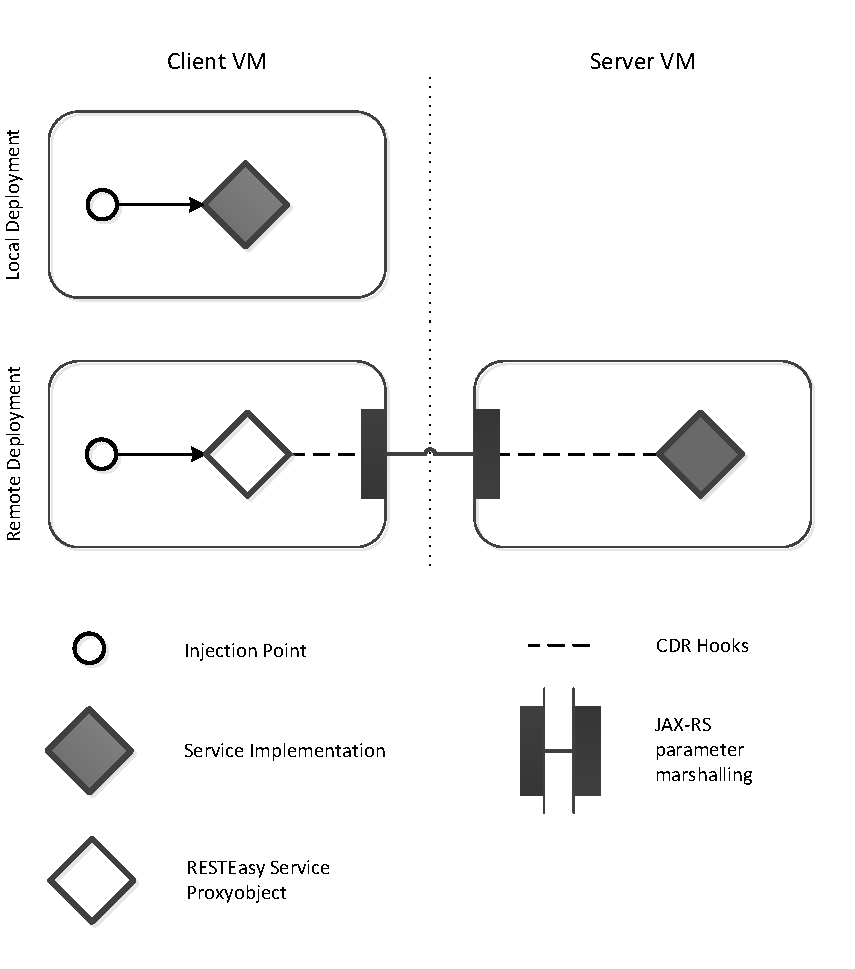
\includegraphics[width=0.8\textwidth]{img/CDR}
\caption{Architektur CDR\label{pic:cdr}}
\end{figure}
Abbildung \ref{pic:cdr} zeigt schematisch die Funktionsweise des \ac{CDR}"=Entwurfsmusters. Der Anwendungsfall wird durch den Beispielode \ref{lst:usecase} aufgezeigt und ist die Verwendung einer Komponente, die die Schnittstelle \textit{Service} implementiert.
\begin{lstlisting}[caption={Anwendungsfall CDR"=Entwurfsmuster},captionpos=b,label=lst:usecase] 
@Inject
Service srv;
...
srv.doSomething();
\end{lstlisting}
Es werden die zwei Bereitstellungsvarianten \textit{Local deployment} und \textit{Remote deployment} unterschieden. 
Die Variante \textit{Local deployment} beschreibt ein Szenario, bei dem die Nutzung und die Breitstellung der \textit{Service}"=Komponente in der selben \ac{JVM} stattfinden. Ein \textit{Remote deployment} liegt demnach vor, wenn die \textit{Service}"=Komponente in einer von der Implementierung entfernten \ac{JVM} genutzt wird.\\ 
Die Variante \textit{Local deployment} ist der Standardfall. 
In der Client"=\ac{JVM} wird eine Implementierung der \textit{Service}"=Schnittstelle bereitgestellt, hier \textit{Service implementation}. 
Der \ac{CDI}"=Mechanismus kann die Abhängigkeiten ohne weitere Informationen auflösen. Es sind keine Anpassungen oder Annotationen am Quellcode notwendig.\\
Bei der Variante \textit{Remote deployment} wird im Beispielcode \ref{lst:usecase} eine Referenz auf ein Stellvertreterobjekt injiziert. 
Dieses Stellvertreterobjekt kommuniziert mit der Implementierung der \textit{Service}"=Komponente, die in der Server"=JVM bereitgestellt wird. 
In beiden \ac{JVM}s bietet das \ac{CDR}-Entwurfsmuster die Möglichkeit eigenen Code auszuführen (\textit{CDR hook}), um die Parameter, Rückgabewerte oder Exceptions nach Bedarf zu transformieren. Dadurch können die in Kapitel \ref{sec:introduction} definierten Ziele wie transparente \textbf{Methodensignaturen} und \textbf{Exceptions} realisiert werden.
Die Kommunikation über die Grenzen der \ac{JVM}s hinweg findet mit Hilfe der \ac{JAX-RS}"=Technologien statt, die auch eine transparente \textbf{Serialisierung} der übertragenen Objekte im \ac{JSON}"= oder \ac{XML}"=Format ermöglichen.
Die Komponenten werden bei dieser Variante auf zwei \ac{JVM}s verteilt. 
Die \textit{Service}"=Schnittstelle und die \ac{CDR}"=Komponenten sind in einer Client"=JVM verfügbar, während eine Server"=JVM die Implementierung der \textit{Service}"=Schnittstelle und die dort notwendigen \textit{CDR hooks} beinhaltet.\\
Die Entscheidung über die Art der Bereitstellung hat keine Auswirkung auf die Anwendungslogik und kann daher für jeden Fall individuell getroffen und im Nachhinein auch wieder geändert werden.
Dadurch dass ein \textit{Local deployment} als Standardfall angenommen wird und alle Änderungen für ein \textit{Remote deployment} nicht die Anwendungslogik berühren, kann das \ac{CDR}"=Entwurfsmuster auch bei Bedarf leicht nachträglich ergänzt werden.
Die notwendigen Anpassungen werden in Kapitel \ref{sec:implementation} aufgezeigt.